\documentclass[../main.tex]{subfiles}

\begin{document}

\section{Movimiento de suelos}

\subsection{Generalidades}

Lo primero que debemos estudiar son dos caracteristicas del suelo: la granulometría
y los límites de Atterberg. Además se deben conocer las caracteristicas geotecnicas
del suelo, tales como la densidad de suelo seco $D_{ss}$, humedad del suelo, 
límite líquido $LL$, límite plástico $LP$ y el índice de plasticidad $IP = LL - LP$.

Conociendo las propiedades anteriores podemos encontrar si el material es granular,
sea canto rodado, grava, arena gruesa o arena fina, o si es un material cohesivo,
sea un limo o una arcilla.

\subsubsection{Límites de Atterberg}

Existen tres límites de Atterberg, que nos permiten clasificar el suelo cohesivo.

\begin{description}
  \item[Límite plástico]  se realiza con la porción de suelo que pasa el tamiz 
    Nº40. Se define como el más bajo contenido de humedad con el que al ser moldeado
    en barritas cilíndricas de menor diámetro cada vez, comienza a agrietarse cuando
    las barritas tienen $\SI{3}{mm}$.

  \item[Límite líquido]  es la menor humedad a partir de la cual el suelo se 
    comporta como un líquido. Se define como el más bajo contenido de humedad para
    que las dos mitades de una pasta de suelo de $\SI{1}{cm}$ de espesor fluyan
    y se unan en una longitud de $\SI{12}{mm}$ en el fondo de la muesca que separa
    las dos mitades cuando la cápsula que la contiene es golpeada 25 veces desde
    una altura de $\SI{1}{cm}$ a dos golpes por segundo.

  \item[Límite de contracción] es la humedad para la cuale el suelo no se contrae
    cuando la humedad baja de ese punto.
\end{description}

\subsubsection{Clasificación de suelos HRB}

Es equivalente al método AASHTO, y cuenta con siete grupos principales, que van
desde el A-1 al A-7. Este método se desarrolló para la construcción de caminos.
Los grupos estan agrupados por granulometría, límite líquido e índice de plasticidad.
También se puede obtener el indice de grupo con la siguiente formula:

\begin{align*}
  IG = (F-35)*(0.2 + 0.005 * (LL - 40)) + 0.01 * (F - 15) * (IP - 10)
.\end{align*}

Donde $F$ es el porcentaje que pasa el tamiz Nº200.

En general, podemos distinguir lo siguiente en cuanto a la calidad de los materiales
para las tareas de caminos:

\begin{itemize}
  \item \textbf{A-1 a A-3:} excelente a buen material para subrasante.
  \item \textbf{A-4 a A-7:} regular a pobre material para subrasante.
\end{itemize}

\subsection{Reconocimiento del terreno}

\subsubsection{Zanjas y calicatas}


Podemos dar como ejemplo las \textbf{calicatas, zanjas y pozos}. Son un sistema
simple y efectivo que nos permite la observación \textit{in situ} del terreno.
Es un méotod válido para profundidades de hasta $\SI{5}{m}$ de profundidad. El
método es ideal para terrenos duros y para arcillas expansivas, ya que permite
la determinación del nivel freático con precisión.
Este tipo de ejecución además requiere entibaciones para $h \geq \SI{1.5}{m}$.

\subsubsection{Sondeos}

Por otro lado tenemos los \textbf{sondeos}, que son perforaciones de pequeño
diámetro y de gran profundidad. Se pueden obtener por rotación, percusión o 
por presión.

Es un requisito un espaciamiento entre auscultaciones de $\SI{500}{m}$ para 
terraplenes y de $\SI{250}{m}$ para desmontes.

\subsection{Compactación}

La compactación consiste en la reducción del volumen del suelo mediante la aplicación
de energía mecánica. Este tema requiere un punto especial de estudio mediante
ensayos como el \textbf{Ensayo Proctor}, que nos permite la elaboración de un
diagrama del que se pueden obtener los valores de la humedad óptima $H_{opt}$
 y la densidad Proctor máxima $\delta_{max}$.

En este tema es importante el concepto de \textbf{valor soporte}, que será definitorio
en la capacidad portante en el suelo como se ve en la imagen.

\begin{figure}[ht]
  \centering
  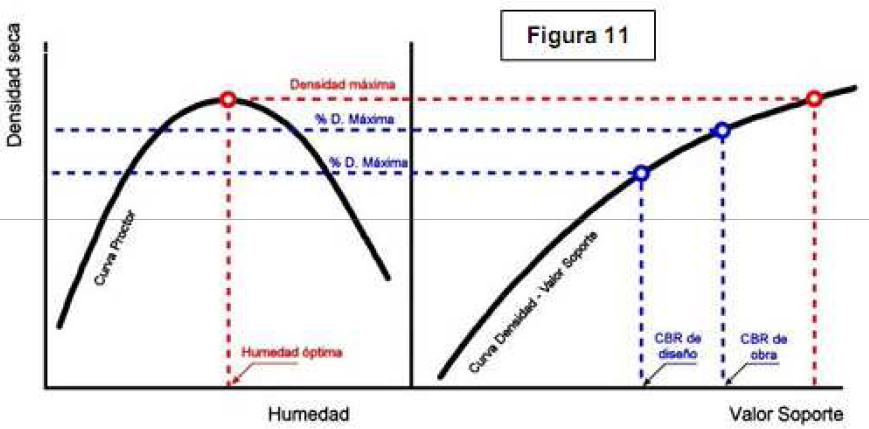
\includegraphics[width=0.8\textwidth]{../images/20210422/valor_soporte}
  \caption{Relación entre Proctor y Valor Soporte}
  \label{fig:valor_soporte}
\end{figure}

Esto muestra las grandes diferencias que pueden llegar a provocar pocos puntos
de diferencia en la densidad deseada en la capacidad de soportar cargas del suelo.

\subsubsection{Control de compactación}

Algunos métodos para la verificación de la compactación de la compactación del
suelo es con el \textit{método del cono de arena}, que consiste en obtener el volumen
de un suelo en el lugar gracias a la comparación con una arena de densidad conocida.

El ensayo se esquematiza en la imagen.

\begin{figure}[ht]
  \centering
  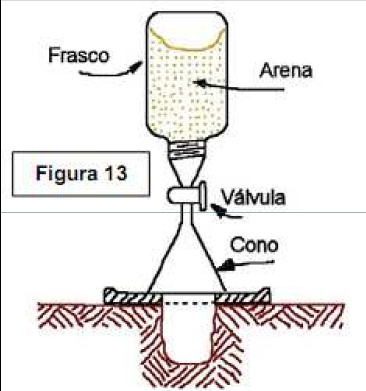
\includegraphics[width=0.4\textwidth]{../images/20210422/cono_arena}
  \caption{Cono de arena}
  \label{fig:cono_arean}
\end{figure}

Sin embargo, también existe otros \textbf{ensayos no destructivos}, como la medición
directa o por retrodispersión.

\subsection{Valor soporte CBR}

El \textbf{CBR} de un suelo es la relación en \% entre el esfuerzo necesario
para penetrar un pistón de dimensiones dadas a una velocidad prefijada hasta una
profundidad determinada en la muestra del suelo analizado y la presión correspondiente
para la penetración en una muestra patrón con caracteristicas ideales. Su valor
depende en gran manera de:

\begin{itemize}
  \item Caracteristicas físico químicas del suelo.
  \item Densidad seca.
  \item  Forma de compactación.
  \item  Humedad con el que fue compactado.
  \item Humedad al momento del ensayo.
  \item Sobrecarga aplicada en el momento del ensayo.
\end{itemize}

En principio, la \textbf{humedad de compactación} generará un cambio significativo
en el valor de CBR, mientras que la \textbf{sobrecarga} aumenta el CBR en los
suelos friccionales.

\subsubsection{Correlación y valores orientativos}

El valor del CBR nos permite hacer las siguiente correlaciones:

\begin{itemize}
  \item Resistencia $kg/cm^2 \approx 100 * \text{CBR}$.
  \item Hinchamiento $\leq 2\%$ no presenta problemas.
  \item Se requieren ciertos valores para el paquete estructural:
    \begin{itemize}
    \item Base: $\text{CBR} \geq 40\%$
    \item Subbase: $\text{CBR} \geq  40\%$
    \item Subrasante buena: $\text{CBR} \sim 8\%$    
    \item Subrasante regular: $1\% \leq \text{CBR} \leq 5\%$
    \end{itemize}
\end{itemize}

\subsubsection{Módulo de reacción de la subrasante $k$}

El módulo de reacción de la subrasante se define como la \textbf{relación} entre
la presión aplicada mediante un plato de sección dada, a la rasante y la penetración
o deflexión resultante. Éste módulo mide la resistencia (o capacidad soporte) del
material de subrasante a ser comprimido bajo la acción de las cargas trasmitidas
al suelo.

Para su determinación, la presión del plato debe ser \textbf{similar} a la utilizar
en el pavimento en servicio. Además, el valor de $k$ dependerá en gran medida
del \textbf{diámetro del plato}.

\subsection{Suelos expansivos}

Los suelos expansivos son aquellos que pueden un cambio en su volumen cuando
varia su humedad. La variación de frecuentes variaciones de humedad de los suelos
de subrasante producen daños severos en los pavimentos que es denominado
\textit{daño silencioso}, y tiene un importante efecto económico.

Este tipo de suelos tiene deformaciones significativamente mas grandes que las 
elásticas, generando un movimiento desigual y causando daños tales como grietas
o quiebres en los pavimentos. En general, el componente arcilloso que provoca esto
es la \textbf{montmorillonita}, que es altamente expansiva. 

Las partículas de arcilla tienen una carga neta negativa, por lo que el agua es
atraída, y a medida que el agua es \textit{adsorbida}, empuja partículas de archilla
causando el hinchamiento.

\subsubsection{Propiedades del suelo}

Las propiedades que pueden afectar esto son:

\begin{description}
  \item[Mineralogía de la arcilla] principalmente la montmorillonita, que genera
    grandes cambios de volumnes.
  \item[Agua química del suelo]
  \item[Succión del suelo] más agua atraída cuando la succión es alta.
  \item[Plasticidad] un alto valor de índice plástico genera más hinchamiento.
  \item[Estructura del suelo] las arcillas dispersivas se expanden con la 
    floculación del suelo.
  \item[Densidad seca] una mayor densidad da a un mayor potencial de hinchamiento.
\end{description}

\subsubsection{Medidas de control}

Ciertas posibilidades para el control de esta problematica son las siguientes:

\begin{enumerate}
  \item Relocalización del trazado.
  \item Reemplazar el suelo expansivo por uno que no lo sea.
  \item Modificar las propiedades expansivas del suelo mediante acciones 
    físicas o químicas.
    \begin{description}
      \item[Físicas] se pueed inundar el suelo de manera que se produzca la
        expansión previa la construcción, o esclarificar, rastrear y agregar arena,
        o en todo caso agregar un revestimiento no expansivo.
      \item[Químicas] estabilización mediante cal, inyecciones, etc.  
    \end{description}
  \item Aislar el suelo de manera que no sufra modificaciones de humedad, tales
    como membranas asfálticas.
\end{enumerate}

El siguiente esquema muestra una solución de impermeabilización de taludes con
arcillas expansivas, como se ve en \Cref{fig:arcillas_expansivas}, \Cref{fig:arcillas_expansivas2}
y \Cref{fig:arcillas_expansivas3}.

\begin{figure}[ht]
  \centering
  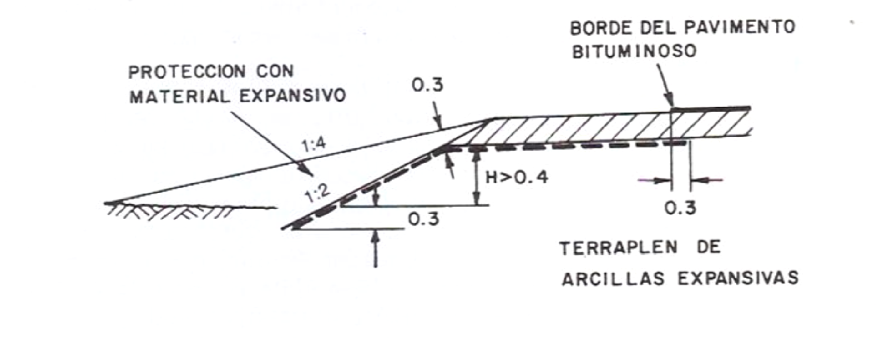
\includegraphics[width=0.8\textwidth]{../images/20210422/arcillas_expansivas}
  \caption{Impermeabilización de taludes en carretera}
  \label{fig:arcillas_expansivas}
\end{figure}

\begin{figure}[ht]
  \centering
  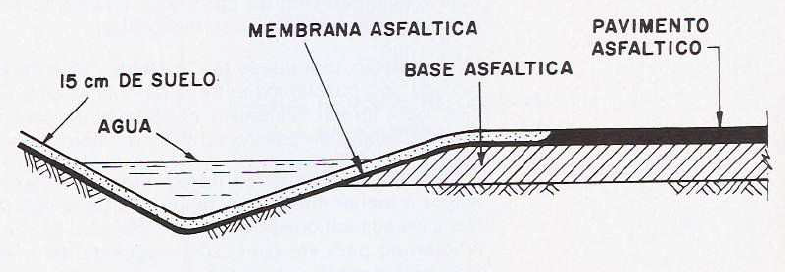
\includegraphics[width=0.8\textwidth]{../images/20210422/arcillas_expansivas2}
  \caption{Impermeabilización de cunetas}
  \label{fig:arcillas_expansivas2}
\end{figure}

\begin{figure}[ht]
  \centering
  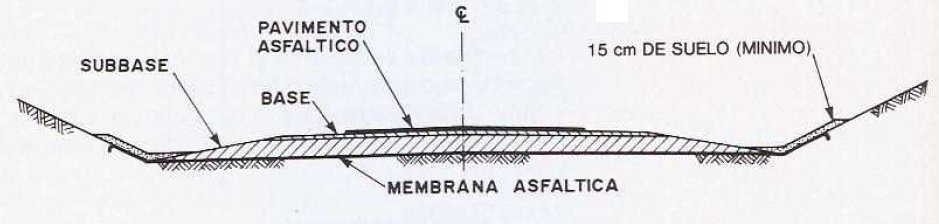
\includegraphics[width=0.8\textwidth]{../images/20210422/arcillas_expansivas3}
  \caption{Impermeabilización de corte tipo}
  \label{fig:arcillas_expansivas3}
\end{figure}

\subsection{Congelamiento de pavimentos}

Las heladas tiene dos efectos perjudiciales en los pavimentos:

\begin{enumerate}
  \item Levantamiento del pavimento por la presión que origina el mayor espacio
    que ocupa el agua congelada.
  \item Ablandamiento de la subrasante por el agua de deshielo.
\end{enumerate}

La profundida de penetración depende de la temperatura bajo el punto de congelamiento
y del tiempo que la misma se mantiene, ya que la transimisión de calor no es 
instantanea, por lo que esto es un problema en lugares donde las bajas temperaturas
se mantienen durante tiempos prolongados.

\subsubsection{Influencia sobre la estructura del suelo}

Se puede dar un proceso de congelación del agua, que mayor volumen en los
espacios entre partículas, desplazando al aire y a las propias partículas en sí.
Luego se da un efecto de \textbf{deshielo}, donde la mayor separación entre partículas
queda de manifiesto, reduciendo la densidad del suelo y reduciendo el valor
soporte del mismo.

Los suelos más susceptibles son los \textbf{suelos finos}, que tienen elevada
capilaridad y baja cohesión, como los suelos limosos o limo-arenosos, mientras
que las arenas y los suelos arcillosos resultan menos sensibles.

\subsubsection{Tratamiento de suelos susceptibles}

Existen varias soluciones para esta problematica, como:

\begin{enumerate}
  \item Retirar el suelo susceptible a las heladas y reemplzarlo por uno no
    susceptible.
  \item Ubicar y compactar el suelo no susceptible con un espesor tal que pueda
    evitar la congelación.
  \item Retirar \textit{bolsones} aislados de suelos susceptibles a las heladas
    para eliminar cambios abruptos.
  \item Aumentar el espesor del pavimento para dar cuenta de la reducción de la 
    capacidad portante durante el deshielo.
  \item Estabilizar el suelo mediante la instalación de una barrera capilar, que 
    pueden ser dos capas de geotextil.
\end{enumerate}

\subsection{Tecnología de áridos}

Son \textbf{rocas} que sufren un proceso de tratamiento industrial para
convertirla en un material granular que tiene una distribución granulométrica
adecuada. Son materiales baratos y abundantes, y luego del agua, la materia
prima más utilizada.

\subsubsection{Áridos naturales}

A este tipo de áridos los podemos dividir en dos tipos:

\begin{description}
  \item[Áridos granulares (rodados)] son aquellos que se obtienen de yacimientos
    naturales (areneros y graveras) y que se usan tras haber sufrido un lavado y
    clasificación. Esto quiere decir que \textit{solo} se modifica su granulometría.

  \item[Áridos de machaqueo] son aquellos que se producen en \textit{canteras}.
    Tras arrancar los materiales de macizos rocosos, se someten a un proceso
    de trituración, molienda y clasificación. 
\end{description}

\subsubsection{Propiedades como elementos granulares}

Podemos distinguir lo siguiente:

\begin{description}
  \item[Propiedades físicas macroscópicas] tales como la dimensión, forma, 
    redondez, densidad, porosidad, permeabilidad, dureza, módulo elástico, 
    conductividad térmica, etc.
  \item[Propiedades químicas] tales ocmo estabilidad mineral, presencia de
    sulfatos y sulfuros, cloruros, etc.
  \item[Propiedades mineralógicas] composición textura, tamaño de grano, 
    cristalinidad, etc.
\end{description}

\subsubsection{Propiedades como conjunto}

\begin{description}
  \item[Composicionales] pueden ser áridos monogénicos y poligénicos. 
  \item[Distribución de tamaños] husos granulométricos.
  \item[Forma] índice de lajas y agujas.
\end{description}

En general, se evaluan \textbf{parametro geométricos}, \textbf{parámetros hidrogeológicos} 
y \textbf{parámetros de material extraible}.

\subsubsection{Rock Quality Designation}

Es un parámetro para medir la calidad de la roca, y depende de la longitud de 
los trozos testigos con una longitud mayor a 10 con respecto a la tirada total
recuperada. La formula es la siguiente:

\begin{align*}
  \text{RQD} = \frac{\Sigma x_{i}}{L}*100
.\end{align*}

Su valor variará de 0 a 100, donde 100 es excelente y 0 es muy malo.

% COMPLETAR
% Desde diapositiva 55 de UT1:05.

\subsection{Rendimiento de los equipos}

\begin{description}
  \item[Comentario 1] los trabajos requieren varios equipos trabajando de forma
    simultanea. El ideal es que todos los equipos trabajen eficazmente y con
    continuidad, pero esto no es fácil, por lo que los valores obtenidos no son
    necesariamente reales. Esto nos indica que los rendimientos calculados de
    forma individual no son valores reales, sino que es necesario encontrar 
    rendimientos para grupos de equipos.

  \item[Comentario 2] la organización de un \textit{kit} de equipo de máquinas
    es el objetivo del ingenierio. Esta situación irá variando durante el transcurso
    de la obra. 

  \item[Comentario 3] las empresas tiene los equipos que tienen. Esto implica que
    nos tenemos que ajustar a los rendimientos de equipos disponibles. 
\end{description}


\href{https://youtu.be/zlrogWSgd9k}{Clase 20210422}


\end{document}
